\chapter{Experimental Results}

\begin{figure*}[pt]
    \centering
    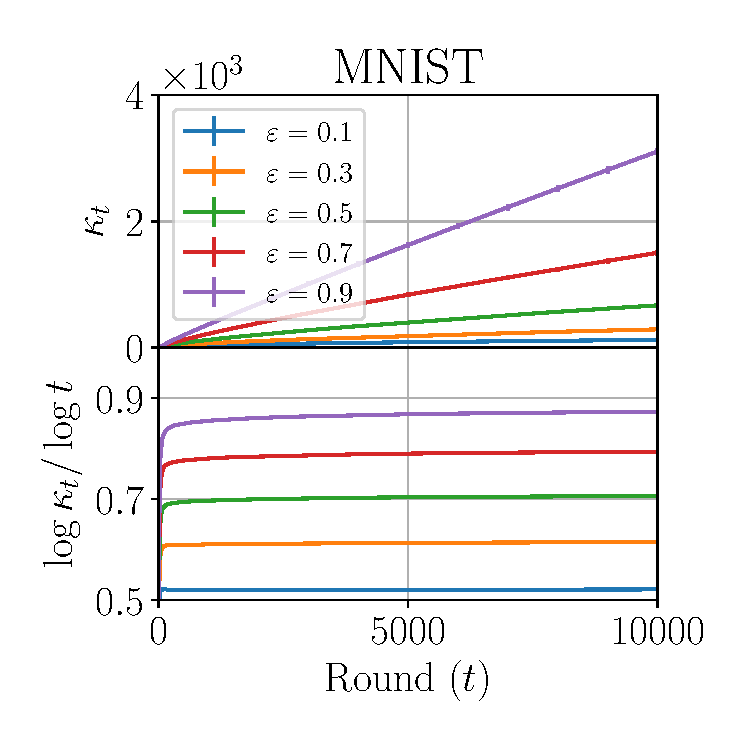
\includegraphics[width=.45\textwidth]{figures/mnist-consistency}%
    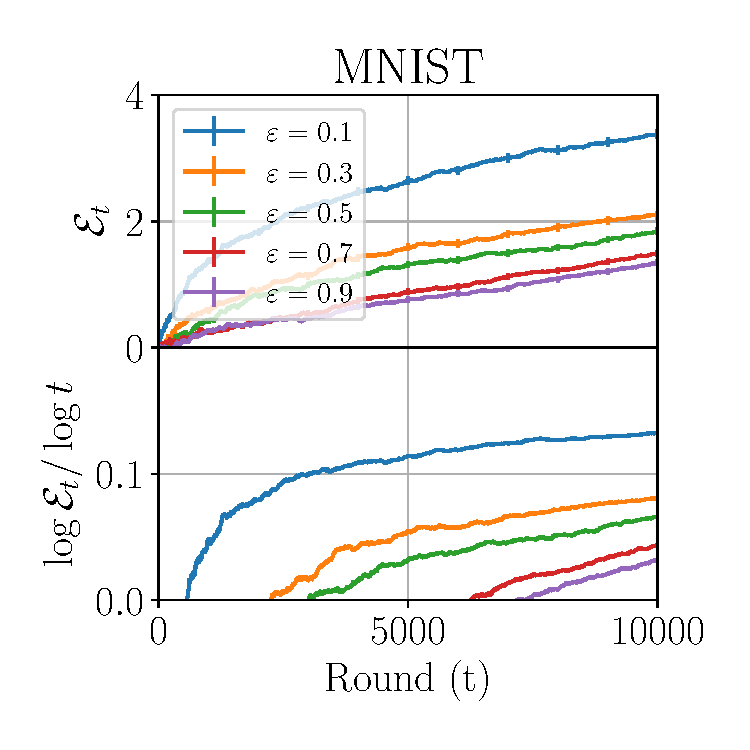
\includegraphics[width=.45\textwidth]{figures/mnist-extra-regret}\\
    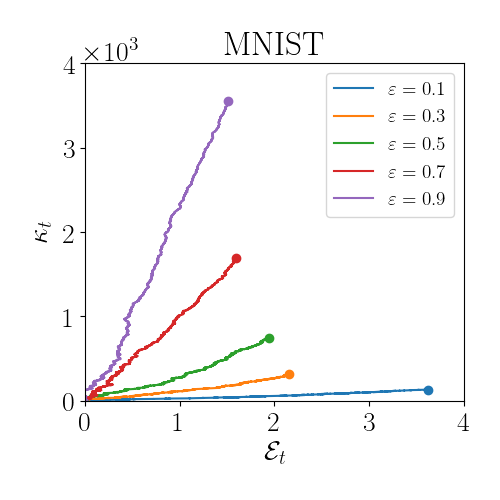
\includegraphics[width=.45\textwidth]{figures/mnist-extra-reg-vs-consistency}%
    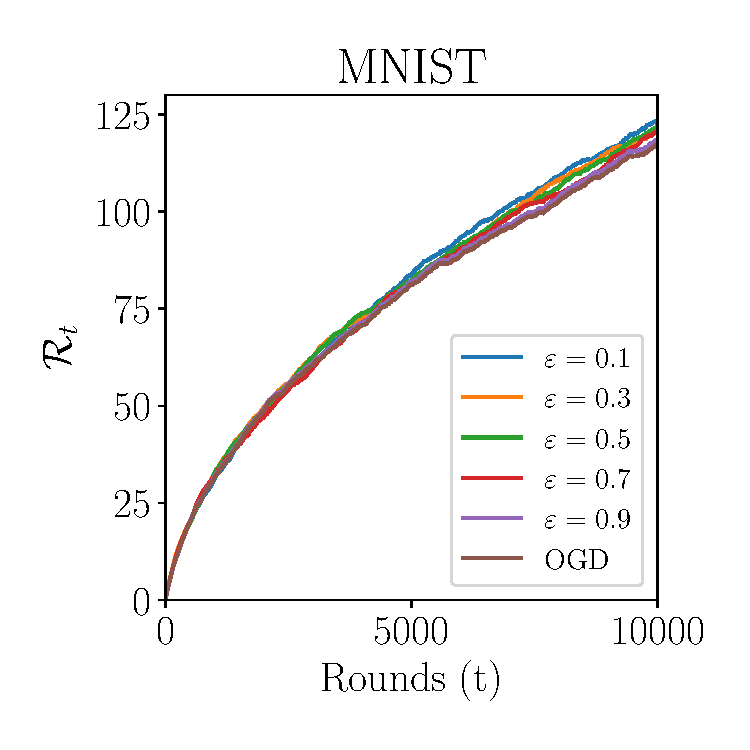
\includegraphics[width=.45\textwidth]{figures/mnist-regret}
     \caption{Experimental results for Online Convex Optimisation on MNIST dataset.}
    \label{fig:experiments1}
\end{figure*}
\begin{figure*}[pt]
    \centering
    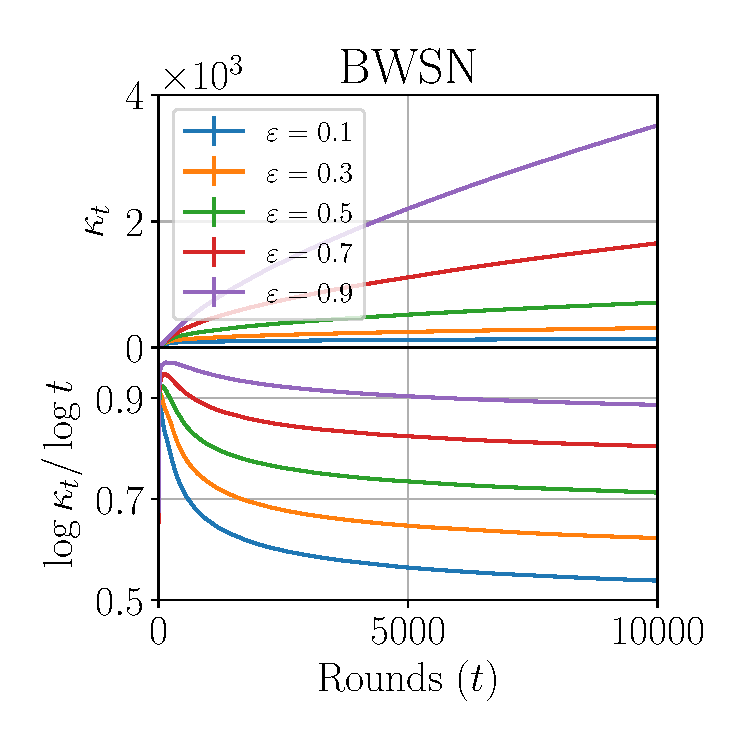
\includegraphics[width=.45\textwidth]{figures/bwsn-consistency}%
    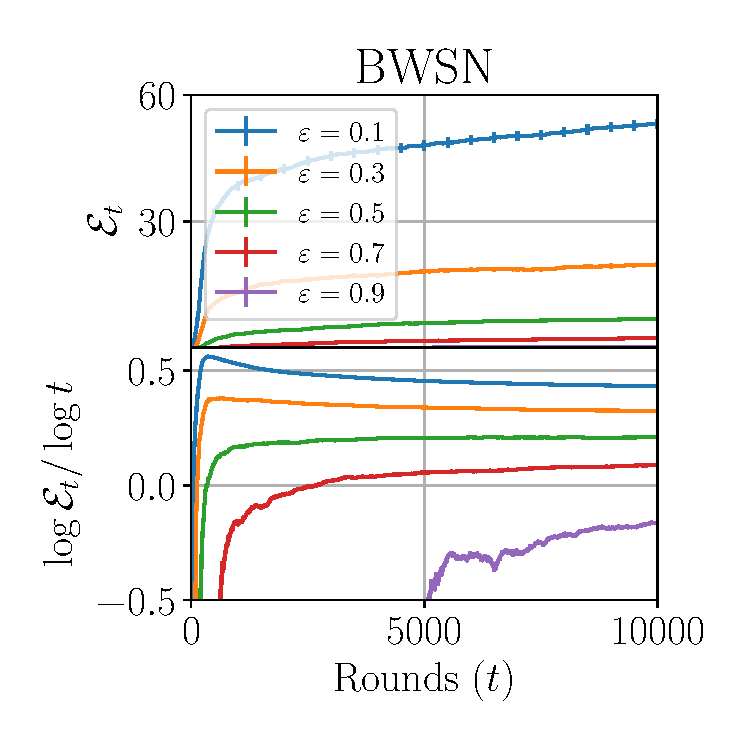
\includegraphics[width=.45\textwidth]{figures/bwsn-extra-regret}\\
    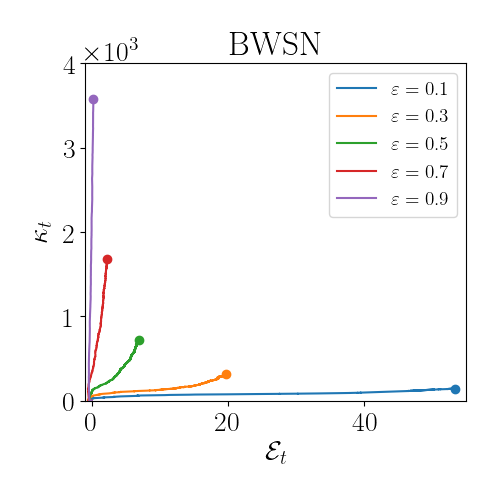
\includegraphics[width=.45\textwidth]{figures/bwsn-extra-reg-vs-consistency}%
    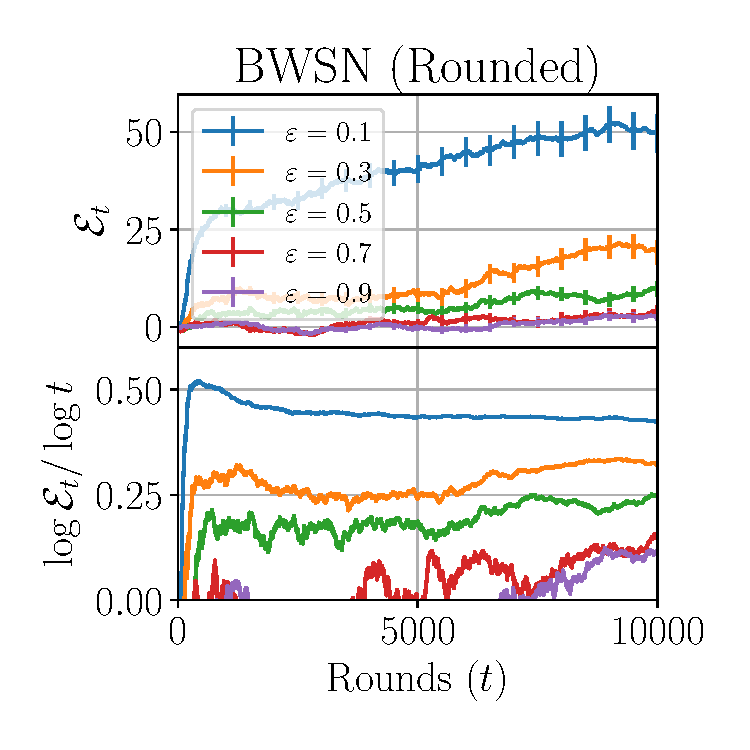
\includegraphics[width=.45\textwidth]{figures/bwsn-extra-regret-rounded}
    \caption{Experimental results for Online Submodular Maximisation for the BWSN problem.}
    \label{fig:experiments2}
\end{figure*}

We evaluate the performance of our algorithm for different parameters of $\varepsilon$, demonstrating different points on the consistency vs. regret trade-off curve. Overall, we find that while the base algorithm $\mathcal{A}$ updates the solution at every time step, overwhelmingly we suffer very little additional regret when we choose to update significantly fewer times. 

\section{Experiments}
We focus on two cases: OCO and Online Submodular Maximisation.
\subsection*{Online Convex Optimisation} We perform Online Logistic Regression on the MNIST dataset of handwritten digits \citep{lecun1998mnist}, to distinguish digit 3 from 5 over the unit $\ell_1$ ball. The training data consists of 11\,552 images labeled with either $1$ or $-1$, and at each round, an image $u$ is selected uniformly at random. The algorithm proposes a vector $w$, and the incurred loss would be
\[
    f(w) = \log(1 + e^{-y\cdot(u^\top w)}),
\]
where $y$ is the label for the image. In this setting, the expected regret is defined as:
\[
    \mathcal{R}_T = \sum_{t=1}^T f_t(x_t) - T\cdot\min_{\|x\|_1 \leq 1} \ev[f(x)],
\]
where the expectation is evaluated over the training set.

\subsection*{Online Submodular Maximisation}
We investigate the problem introduced in the Battle of the Water Sensor Networks challenge \citep{ostfeld08bwsn}, where the goal is to find the best set of sensor locations to detect a contamination event, minimising detection time.

In our experiment, we select 20 sensors from among 12\,527 possible locations, based on performance on a set of contamination events.  As \citet{leskovec07cost} showed, this problem can be formulated as an instance of the facility location problem: For any subset of sensor locations $S$, every contamination event is a submodular function $f_e(S) := \max_{s\in S} w_{e,s}$, where $w_{e,s}$ is the reduction in penalty for sensor $s$ in event $e$. Given that the events are sampled from some distribution $\Dcal$, the optimisation problem can be written as
\[
    \max_{S\subseteq V, |S|\leq 20} \EE_{f\sim \Dcal}[f(S)].
\]

We perform Online Gradient Ascent on the multilinear extension of $f_e$'s, which can be computed easily (\cf, \citet[Appendix E.2]{Karimi2017}). The optimisation domain is the matroid base polytope for the cardinality constraint.

In this setting we cannot compute the exact  $\frac{1}{2}$-regret. Instead, we compute the extra regret $\Ecal_t$, as well as cumulative utility. We also report results in the case that one rounds the continuous solutions to discrete sets in each round. 

\section{Metrics}
To evaluate the performance of the algorithms we plot the following quantities:
\begin{enumerate}\itemsep=0in
\item Consistency cost, $\kappa_t$, denoting the number of switches in the solution up to time $t$. 
\item Extra regret, $\mathcal{E}_t$, denoting the loss in regret over using the best low-regret algorithm. 
\item For the MNIST dataset, total regret $\mathcal{R}_t$.
\end{enumerate}

Additionally, for consistency and extra regret, we evaluate the growth of the two quantities as a function of $t$. To do so, we plot the functions $\log \kappa_t / \log t$ and $\log \mathcal{E}_t / \log t$ . Observe that if for a function $x$ it holds $x(t) = O(t^{\alpha})$ then $\limsup_{t\to\infty} \frac{\log x(t)}{\log t} \leq \alpha$. This allows us to estimate how close our empirical results are to the theoretical bounds. 

\section{Results}
In Figure~\ref{fig:experiments1} we show the results for the MNIST dataset. In the first panel we plot the consistency cost, showing both the raw cost $\kappa_t$, as well as the scaled version $\log \kappa_t / \log t$. The results closely track those predicted by the theory, as we see $\kappa$ grow as $T^{\frac{1}{2} + \frac{\epsilon}{2}}$. In the second panel we plot the extra regret. Here we see that the theoretical results are overly pessimistic, and the actual extra regret that is achieved is far lower than that predicted by the theory. This leads us to very favorable trade-offs, for instance by taking $\varepsilon=0.3$, the regret increase is less than $2\%$, but the number of updates drops by $30$x over the baseline, as we update on approximately $3\%$ of the rounds. This is further demonstrated in the fourth panel, which shows the total regret of the different parameter settings. The fact that the lines are bunched close together again demonstrates that the additional regret incurred by not updating during the majority of the timesteps is minimal. 

In Figure~\ref{fig:experiments2} we plot the results for the BWSN problem. Here again, in the first panel we investigate the consistency cost where we observe it be sublinear in the number of rounds. In the second panel we plot the extra regret, $\mathcal{E}_t$. Again, the extra regret is far lower than the pessimistic theoretical bound. Moreover, we see that sufficiently high, but bounded away from 1, values of $\varepsilon$, e.g.,  $\varepsilon = 0.9$, appear to lead to an {\em improvement} in results, suggesting that the lack of updating acts as a regularizer. (We note that the improvement is statistically significant.) This improvement is especially pronounced in the fourth plot, where we show the regret due to rounded solutions. Moreover, one can verify the analysis in Section~\ref{sec:submodapplication}, that the regret bound for the multilinear extension upper bounds the regret bound for discrete submodular function. Concretely, by updating in $3\%$ of the rounds, we only suffer $0.3\%$ additional regret, when using $\varepsilon = 0.3$ and rounding the solution.

%Also in both cases, we have plotted the function $\log \Ecal_t / \log t$ and $\log \kappa_t / \log t$ to match our asymptotic results with practice. This plot is based on the fact that if $a_t = O(t^\alpha)$, then 
%\[
%    \limsup_{t\to\infty} \frac{\log a_t}{\log t} \leq \alpha.
%\]

